\documentclass[oneside, a4paper, 12pt]{article}

\usepackage[utf8]{inputenc}
\usepackage[russian]{babel}

\usepackage{misccorr}
\usepackage{indentfirst}

\usepackage{setspace}
\onehalfspace

\usepackage{graphicx}

\usepackage{listings}
\lstset{captionpos=b}

\begin{document}

\tableofcontents
\pagebreak

\section{Введение}

В различных областях науки и техники довольно часто встречается
задача определения схожести строк. Для её решения применяют
разнообразные метрики, наиболее распространёнными из которых
являются расстояния Левенштейна и Дамерау-Левенштейна.

Расстояние Левенштейна определяется как минимальное количество
редакционных операций, необходимых для превращения одной строки в
другую.

Редакционные операции -- это следующие действия над одним символом:

\begin{itemize}
    \item вставка;
    \item удаление;
    \item замена.
\end{itemize}

$$
D_{\textup{Левенштейна}}() = \min
$$

В свою очередь, расстояние Дамерау-Левенштейна учитывает то
обстоятельство, что наиболее частой ошибкой при наборе текстов на
клавиатуре является перестановка (транспозиция) двух символов.
Таким образом, редакционные операции для расстояния
Дамерау-Левенштейна:

\begin{itemize}
    \item вставка;
    \item удаление;
    \item замена;
    \item перестановка.
\end{itemize}

$$
D_{\textup{Дамерау-Левенштейна}}()
$$

\section{Аналитическая часть}

Цель данной работы - изучить метод динамического программирования
на примере реализации алгоритмов поиска расстояний Левенштейна и
Дамерау-Левенштейна.

Для этого необходимо решить следующие задачи:

\begin{enumerate}
    \item изучить расстояния Левенштейна и Дамерау-Левенштейна;
    \item разработать алгоритмы поиска изученных расстояний;
    \item реализовать разработанные алгоритмы;
    \item выполнить оценку затрат реализаций алгоритмов по памяти;
    \item выполнить замеры процессорного времени работы реализаций;
    \item выполнить сравнительный анализ следующих алгоритмов:
    \begin{itemize}
        \item нерекурсивных поиска расстояния Левенштейна и
            нерекурсивного поиска расстояния Дамерау-Левенштейна;
        \item поиска расстояния Дамерау-Левенштейна;
    \end{itemize}
\end{enumerate}

\section{Конструкторская часть}

\subsection{Поиск расстояния Левенштейна}

\subsubsection{Нерекурсивный алгоритм}

Пусть $s$ и $t$ -- строки из $m$ и $n$ символов соответственно,
тогда $D$ -- целочисленная матрица $(m + 1) \times (n + 1)$
элементов, причём $d_{ij}$ -- расстояние Левенштейна между срезами
$(s_k | k \in [1; i - 1])$ и $(t_k | k \in [1; j - 1])$.

Матрица $D$ может быть вычислена с помощью двух вложенных циклов.

\subsection{Поиск расстояния Дамерау-Левенштейна}

\subsubsection{Нерекурсивный алгоритм}

\subsubsection{Простой рекурсивный алгоритм}

Расстояние Дамерау-Левенштейна также может быть вычислено
непосредственно по формуле с помощью рекурсивных функций.

\subsubsection{Рекурсивный алгоритм с кэшем}

\section{Технологическая часть}

\subsection{Средства разработки}

Для реализации разработанных алгоритмов был выбран язык
программирования Rust, поскольку он предоставляет высокую степень
контроля за ошибками во время компиляции.

Также для разработки, тестирования и отладки программ был
использован инструмент Cargo, поскольку он позволяет
автоматизировать значительную часть работы.

Для замера процессорного времени был выбран крейт cpu-time,
поскольку он предоставляет простой и идиоматичный интерфейс.

\subsection{Реализация алгоритмов}

Далее представлен листинг реализации нерекурсивного алгоритма
поиска расстояния Левенштейна.

\begin{lstlisting}[caption=
    Нерекурсивная реализация алгоритма поиска расстояния
    Левенштейна.
]
fn distance(s: &str, t: &str) -> usize {
    let (m, n) = (s.len(), t.len());

    // A matrix of Levenshtein distances
    let mut matrix = Matrix::new(0, m + 1, n + 1);

    for i in 0..m + 1 {
        for j in 0..n + 1 {
            if i == 0 {
                matrix.set(0, j, j);
                continue;
            }

            if j == 0 {
                matrix.set(i, 0, i);
                continue;
            }

            // The current characters
            let c = s.chars().nth(i - 1).unwrap();
            let d = t.chars().nth(j - 1).unwrap();

            let mut cases = vec![matrix.get(i - 1, j - 1)
                + if c == d { 0 } else { 1 }];

            cases.push(matrix.get(i - 1, j) + 1);
            cases.push(matrix.get(i, j - 1) + 1);

            matrix.set(i, j, *cases.iter().min().unwrap());
        }
    }

    *matrix.get(m, n)
}
\end{lstlisting}

В свою очередь, листинг нерекурсивного алгоритма поиска расстояния
Дамерау-Левенштейна имеет следующий вид.

\begin{lstlisting}[caption=
    Нерекурсивная реализация алгоритма поиска расстояния
    Дамерау-Левенштейна.
]
fn distance(s: &str, t: &str) -> usize {
    let (m, n) = (s.len(), t.len());

    // A matrix of Damerau-Levenshtein distances
    let mut matrix = Matrix::new(0, m + 1, n + 1);

    for i in 0..m + 1 {
        for j in 0..n + 1 {
            if i == 0 {
                matrix.set(0, j, j);
                continue;
            }

            if j == 0 {
                matrix.set(i, 0, i);
                continue;
            }

            // The current characters
            let c = s.chars().nth(i - 1).unwrap();
            let d = t.chars().nth(j - 1).unwrap();

            let mut cases = vec![matrix.get(i - 1, j - 1)
                + if c == d { 0 } else { 1 }];

            cases.push(matrix.get(i - 1, j) + 1);
            cases.push(matrix.get(i, j - 1) + 1);

            if i > 1 && j > 1 {
                // The previous characters
                let p = s.chars().nth(i - 2).unwrap();
                let q = t.chars().nth(j - 2).unwrap();

                if c == q && p == d {
                    cases.push(matrix.get(i - 2, j - 2) + 1);
                }
            }

            matrix.set(i, j, *cases.iter().min().unwrap());
        }
    }

    *matrix.get(m, n)
}
\end{lstlisting}

Листинг простой рекурсивной реализации алгоритма поиска расстояния
Дамерау-Левенштейна демонстрирует наглядность такого подхода.

\begin{lstlisting}[caption=
    Простая рекурсивная реализация алгоритма поиска расстояния
    Дамерау-Левенштейна.
]
fn distance(s: &str, t: &str) -> usize {
    let (m, n) = (s.len(), t.len());

    if m == 0 {
        return n;
    }

    if n == 0 {
        return m;
    }

    // The last characters
    let c = s.chars().nth(m - 1).unwrap();
    let d = t.chars().nth(n - 1).unwrap();

    let mut cases = vec![Self::distance(&s[..m - 1], &t[..n - 1])
        + if c == d { 0 } else { 1 }];

    cases.push(Self::distance(&s[..m - 1], t) + 1);
    cases.push(Self::distance(s, &t[..n - 1]) + 1);

    if m > 1 && n > 1 {
        // The last but one characters
        let p = s.chars().nth(m - 2).unwrap();
        let q = t.chars().nth(n - 2).unwrap();

        if c == q && p == d {
            cases.push(Self::distance(&s[..m - 2], &t[..n - 2]) + 1);
        }
    }

    *cases.iter().min().unwrap()
}
\end{lstlisting}

\subsection{Тестирование}

\begin{lstlisting}[caption=Тесты алгоритмов поиска расстояния Левенштейна]
// Both strings are empty
assert_eq!(distance("", ""), 0);

// The first string is empty
assert_eq!(distance("", "right"), 5);

// The second string is empty
assert_eq!(distance("left", ""), 4);

// One insertion is required
assert_eq!(distance("word", "world"), 1);

// One deletion is required
assert_eq!(distance("clock", "lock"), 1);

// One replacement is required
assert_eq!(distance("ping", "pong"), 1);

// One transposition is required
assert_eq!(distance("vse", "sve"), 2);

// Both strings are the same
assert_eq!(distance("zug", "zug"), 0);

// Both strings are different
assert_eq!(distance("heaven", "hell"), 4);
\end{lstlisting}

\begin{lstlisting}[caption=Тесты реализаций алгоритмов поиска расстояния Дамерау-Левенштейна]
// Both strings are empty
assert_eq!(distance("", ""), 0);

// The first string is empty
assert_eq!(distance("", "right"), 5);

// The second string is empty
assert_eq!(distance("left", ""), 4);

// One insertion is required
assert_eq!(distance("word", "world"), 1);

// One deletion is required
assert_eq!(distance("clock", "lock"), 1);

// One replacement is required
assert_eq!(distance("ping", "pong"), 1);

// One transposition is required
assert_eq!(distance("vse", "sve"), 1);

// Both strings are the same
assert_eq!(distance("zug", "zug"), 0);

// Both string are different
assert_eq!(distance("heaven", "hell"), 4);
\end{lstlisting}

\section{Экспериментальная часть}

\subsection{Замеры процессорного времени}

Были проведены замеры процессорного времени работы реализации
каждого алгоритма. Полученные данные представлены в виде графиков.

\begin{figure}[ht]
    \centering
    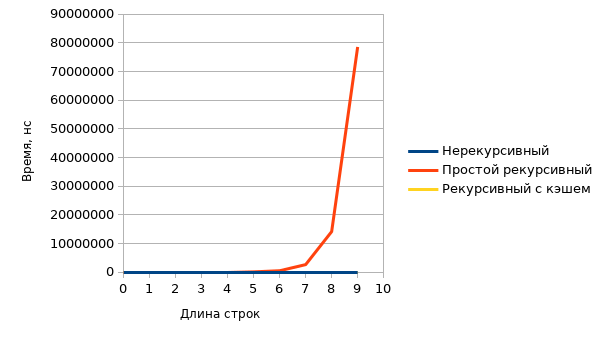
\includegraphics[width=\textwidth]{plt-01.png}
    \caption{Сравнение времени работы реализаций трёх алгоритмов}
\end{figure}

\begin{figure}[ht]
    \centering
    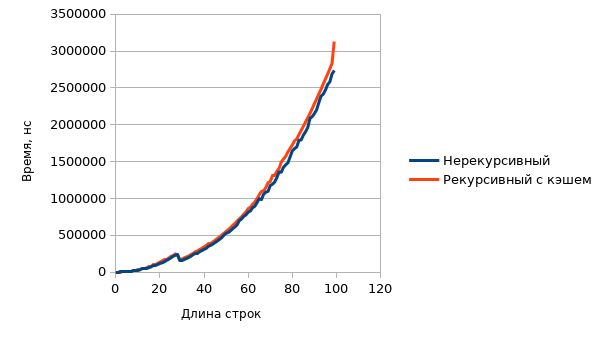
\includegraphics[width=\textwidth]{plt-02.png}
    \caption{Сравнение времени работы реализаций двух алгоритмов}
\end{figure}

\subsection{Выводы}

\section{Заключение}

В ходе работы были решены следующие задачи:

\begin{enumerate}
    \item изучены расстояния Левенштейна и Дамерау-Левенштейна;
    \item разработаны алгоритмы поиска изученных расстояний;
    \item реализованы разработанные алгоритмы;
    \item выполнены оценки затрат реализаций алгоритмов по памяти;
    \item выполнены замеры процессорного времени работы реализаций;
    \item выполнен сравнительный анализ следующих алгоритмов:
    \begin{itemize}
        \item нерекурсивного поиска расстояния Левенштейна и
            нерекурсивного поиска расстояния Дамерау-Левенштейна;
        \item поиска расстояния Дамерау-Левенштейна;
    \end{itemize}
\end{enumerate}

TODO: выводы

\section{Список литературы}

1. Левенштейн, В. И. Двоичные коды с исправлением выпадений,
вставок и замещений символов. / В. И. Левенштейн // Доклады
Академий Наук СССР. -- 1965. -- 163.4. -- 845-848.

2. Damerau, F. J. A technique for computer detection and correction
of spelling errors. / F. J. Damerau // Communications of the ACM.
-- 1964. -- 7 (3). -- 171-176.

\end{document}
